\documentclass{subfile}

\begin{document}
  \section{Appendix}
  \begin{figure}[h!]
  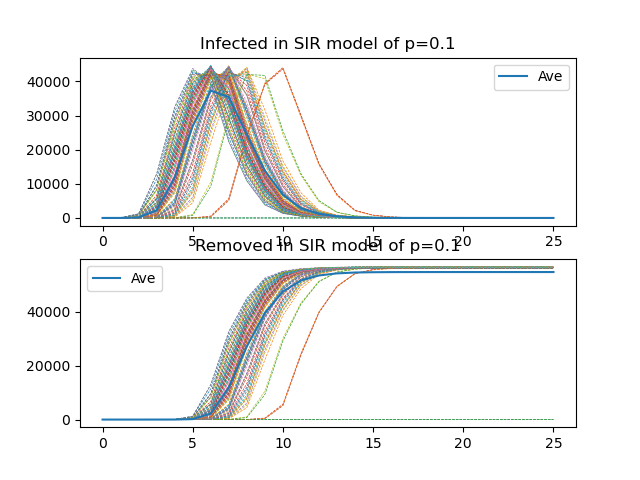
\includegraphics[scale=0.8]{sirp01r1i3s3}
  \caption[SIR p=0.1,r=1,i=3,init infected=3]{SIR Model with p=0.1 r=1 i=3 initial infected=3 simulation using Snap.py}
  \end{figure}
  \begin{figure}
  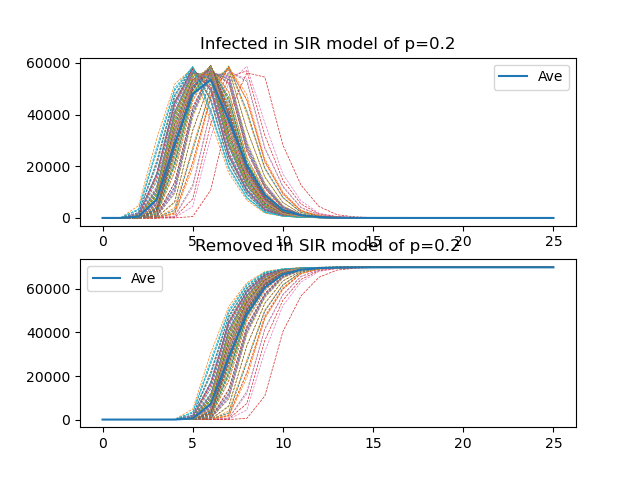
\includegraphics[scale=0.8]{sirp02r1i3s3}
  \caption[SIR p=0.2,r=1,i=3,init infected=3]{SIR Model with p=0.2 r=1 i=3 initial infected=3 simulation using Snap.py}
  \end{figure}
  \begin{figure}
  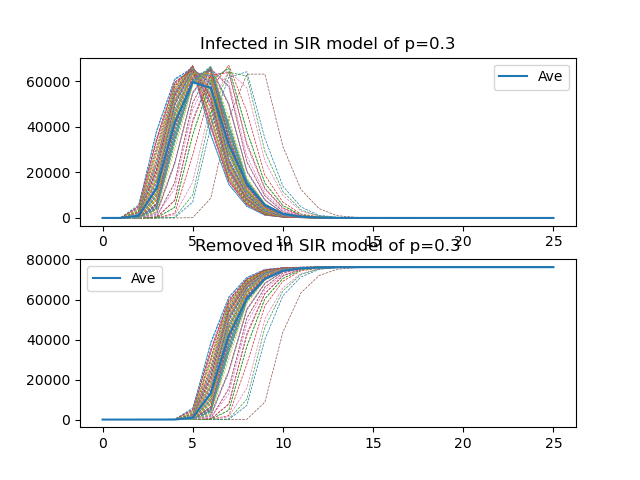
\includegraphics[scale=0.8]{sirp03r1i3s3}
  \caption[SIR p=0.3,r=1,i=3,init infected=3]{SIR Model with p=0.3 r=1 i=3 initial infected=3 simulation using Snap.py}
  \end{figure}
  \begin{figure}
  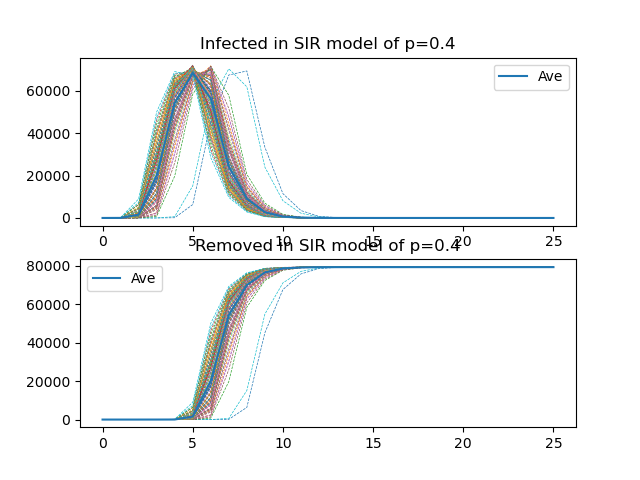
\includegraphics[scale=0.8]{sirp04r1i3s3}
  \caption[SIR p=0.4,r=1,i=3,init infected=3]{SIR Model with p=0.4 r=1 i=3 initial infected=3 simulation using Snap.py}
  \end{figure}
  \begin{figure}
  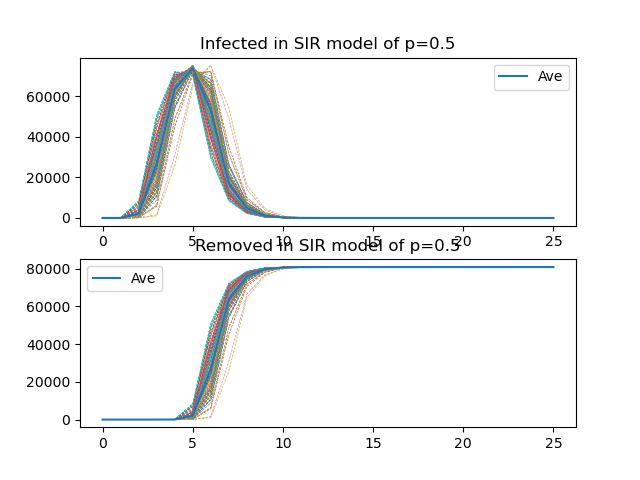
\includegraphics[scale=0.8]{sirp05r1i3s3}
  \caption[SIR p=0.5,r=1,i=3,init infected=3]{SIR Model with p=0.5 r=1 i=3 initial infected=3 simulation using Snap.py}
  \end{figure}
  \begin{figure}
  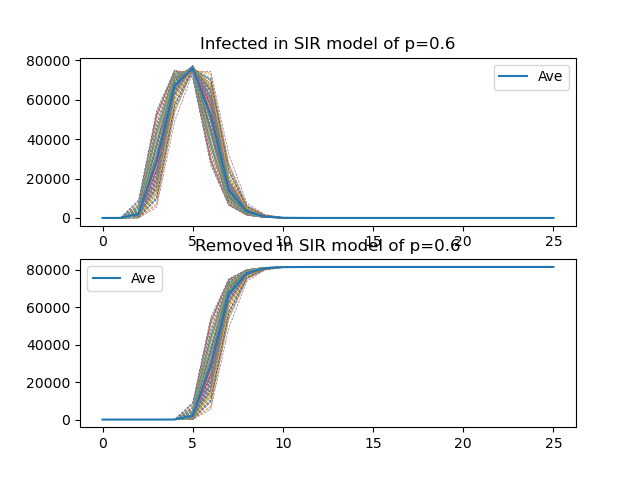
\includegraphics[scale=0.8]{sirp06r1i3s3}
  \caption[SIR p=0.6,r=1,i=3,init infected=3]{SIR Model with p=0.6 r=1 i=3 initial infected=3 simulation using Snap.py}
  \end{figure}
  \begin{figure}
  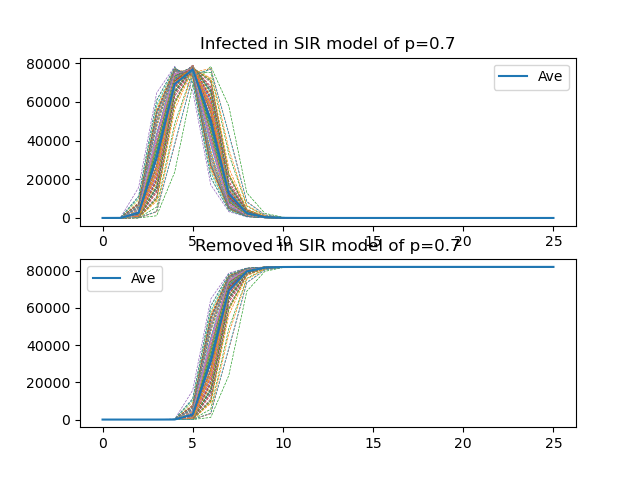
\includegraphics[scale=0.8]{sirp07r1i3s3}
  \caption[SIR p=0.7,r=1,i=3,init infected=3]{SIR Model with p=0.7 r=1 i=3 initial infected=3 simulation using Snap.py}
  \end{figure}
  \begin{figure}
  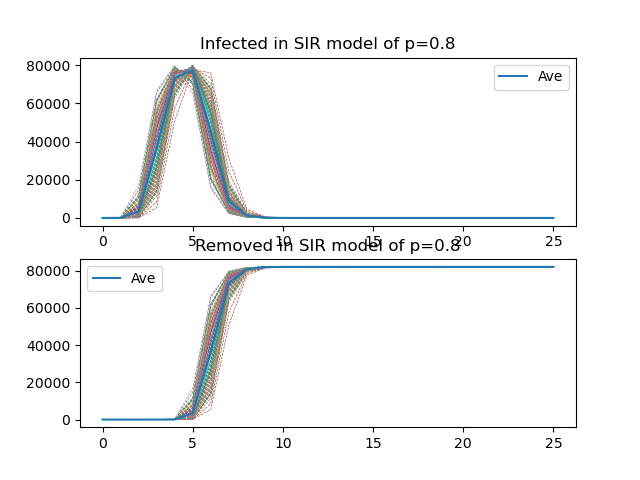
\includegraphics[scale=0.8]{sirp08r1i3s3}
  \caption[SIR p=0.8,r=1,i=3,init infected=3]{SIR Model with p=0.8 r=1 i=3 initial infected=3 simulation using Snap.py}
  \end{figure}
  \begin{figure}
  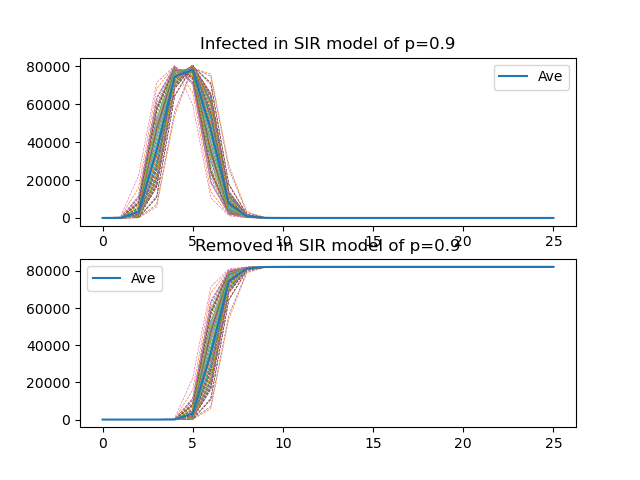
\includegraphics[scale=0.8]{sirp09r1i3s3}
  \caption[SIR p=0.9,r=1,i=3,init infected=3]{SIR Model with p=0.9 r=1 i=3 initial infected=3 simulation using Snap.py}
  \end{figure}
  \begin{figure}
  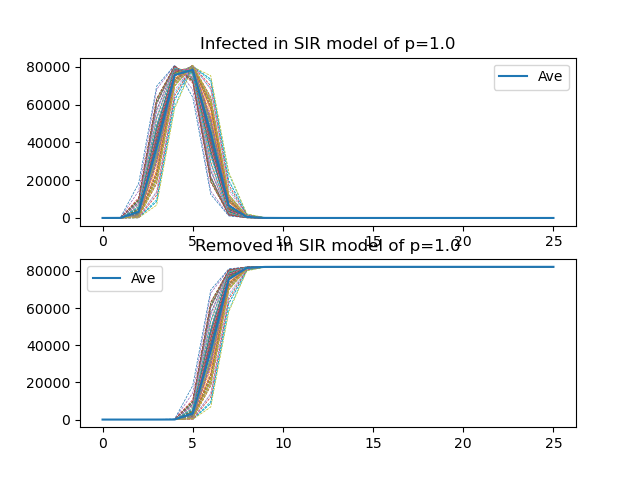
\includegraphics[scale=0.8]{sirp10r1i3s3}
  \caption[SIR p=1.0,r=1,i=3,init infected=3]{SIR Model with p=1.0 r=1 i=3 initial infected=3 simulation using Snap.py}
  \end{figure}
  \begin{figure}
  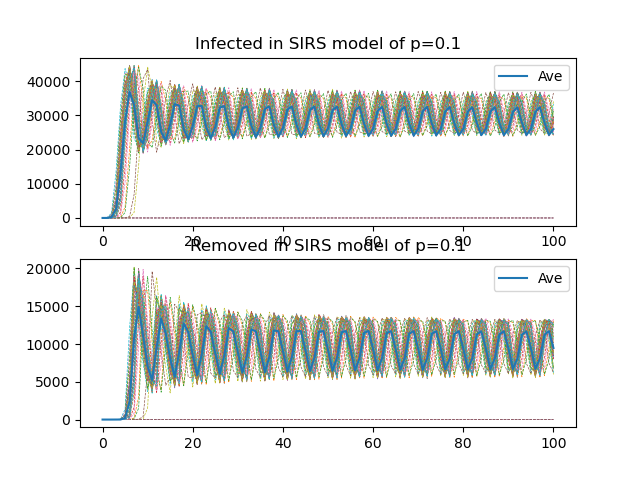
\includegraphics[scale=0.8]{sirsp01r1i3s3}
  \caption[SIRS p=0.1,r=1,i=3,init infected=3]{SIRS Model with p=0.1 r=1 i=3 initial infected=3 simulation using Snap.py}
  \end{figure}
  \begin{figure}
  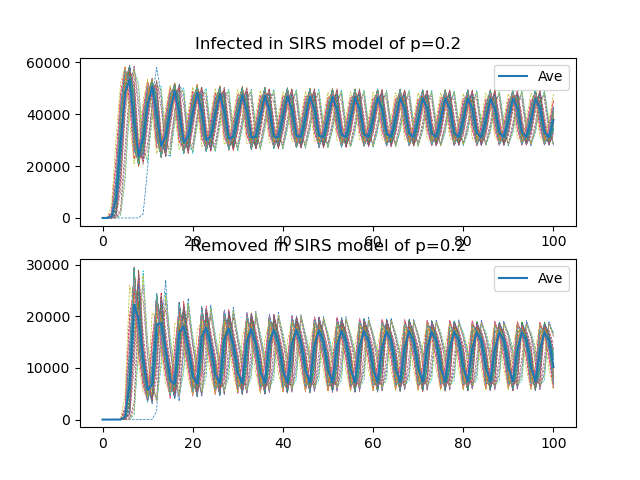
\includegraphics[scale=0.8]{sirsp02r1i3s3}
  \caption[SIRS p=0.2,r=1,i=3,init infected=3]{SIRS Model with p=0.2 r=1 i=3 initial infected=3 simulation using Snap.py}
  \end{figure}
  \begin{figure}
  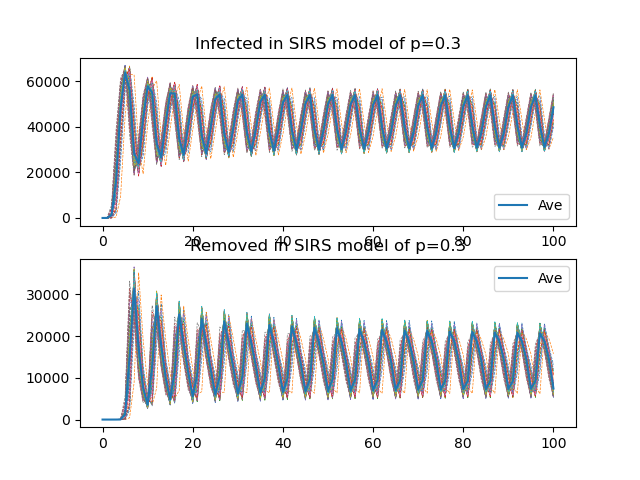
\includegraphics[scale=0.8]{sirsp03r1i3s3}
  \caption[SIRS p=0.3,r=1,i=3,init infected=3]{SIRS Model with p=0.3 r=1 i=3 initial infected=3 simulation using Snap.py}
  \end{figure}
  \begin{figure}
  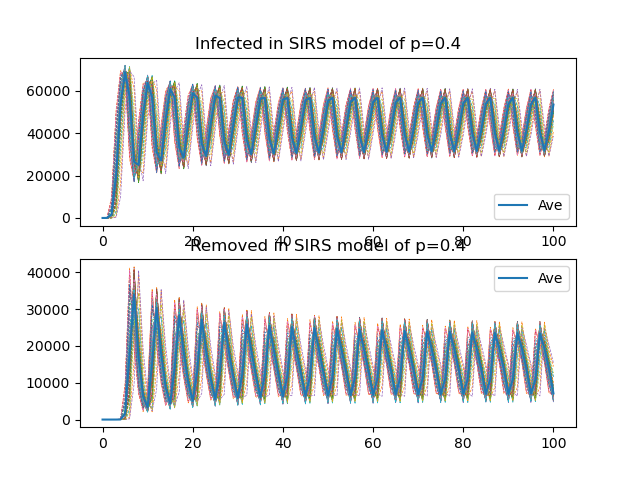
\includegraphics[scale=0.8]{sirsp04r1i3s3}
  \caption[SIRS p=0.4,r=1,i=3,init infected=3]{SIRS Model with p=0.4 r=1 i=3 initial infected=3 simulation using Snap.py}
  \end{figure}
  \begin{figure}
  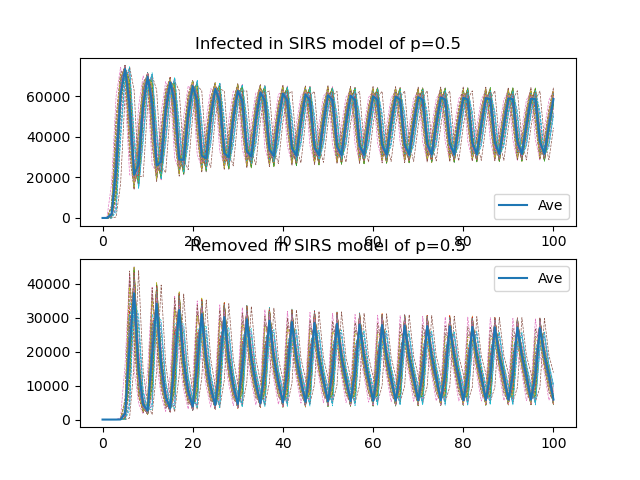
\includegraphics[scale=0.8]{sirsp05r1i3s3}
  \caption[SIRS p=0.5,r=1,i=3,init infected=3]{SIRS Model with p=0.5 r=1 i=3 initial infected=3 simulation using Snap.py}
  \end{figure}
  \begin{figure}
  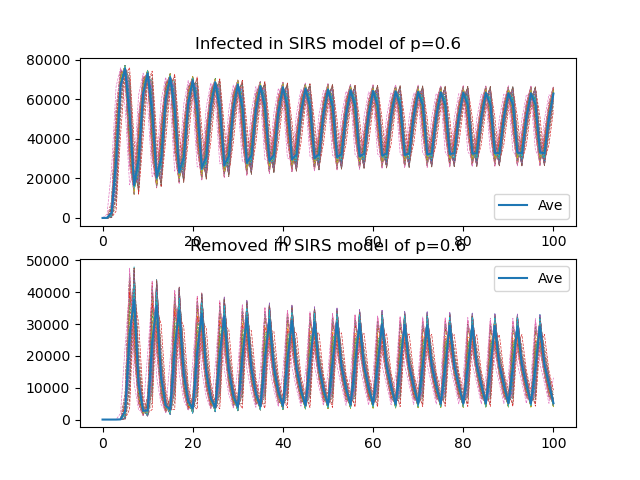
\includegraphics[scale=0.8]{sirsp06r1i3s3}
  \caption[SIRS p=0.6,r=1,i=3,init infected=3]{SIRS Model with p=0.6 r=1 i=3 initial infected=3 simulation using Snap.py}
  \end{figure}
  \begin{figure}
  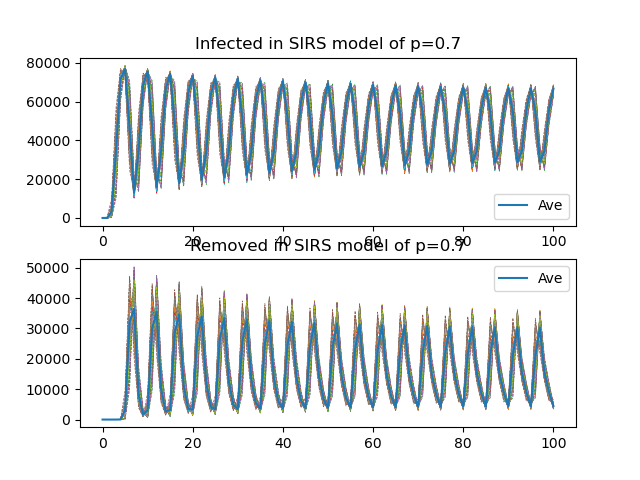
\includegraphics[scale=0.8]{sirsp07r1i3s3}
  \caption[SIRS p=0.7,r=1,i=3,init infected=3]{SIRS Model with p=0.7 r=1 i=3 initial infected=3 simulation using Snap.py}
  \end{figure}
  \begin{figure}
  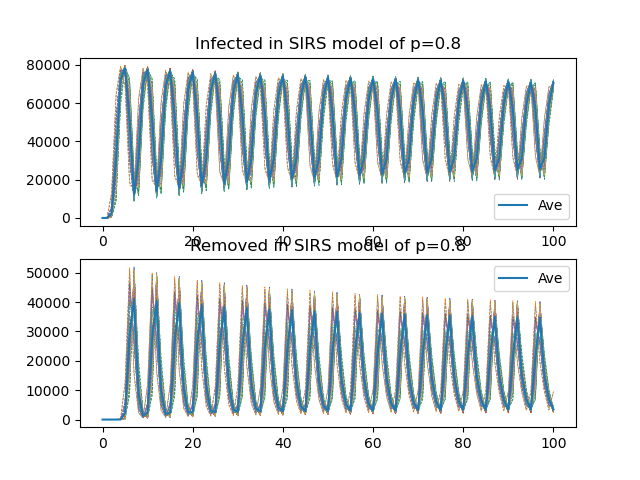
\includegraphics[scale=0.8]{sirsp08r1i3s3}
  \caption[SIRS p=0.8,r=1,i=3,init infected=3]{SIRS Model with p=0.8 r=1 i=3 initial infected=3 simulation using Snap.py}
  \end{figure}
  \begin{figure}
  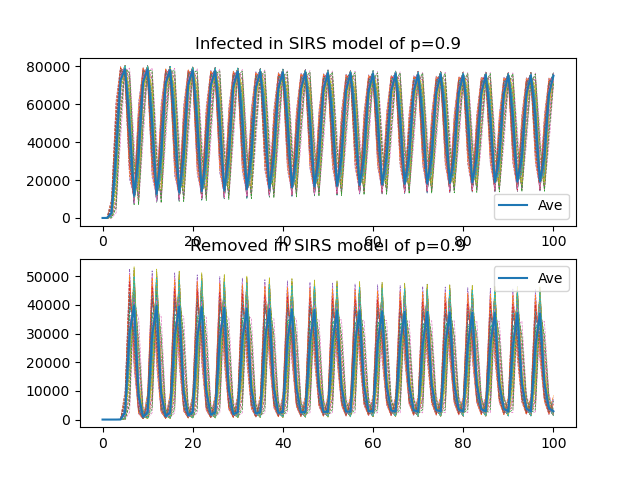
\includegraphics[scale=0.8]{sirsp09r1i3s3}
  \caption[SIRS p=0.9,r=1,i=3,init infected=3]{SIRS Model with p=0.9 r=1 i=3 initial infected=3 simulation using Snap.py}
  \end{figure}
  \begin{figure}
  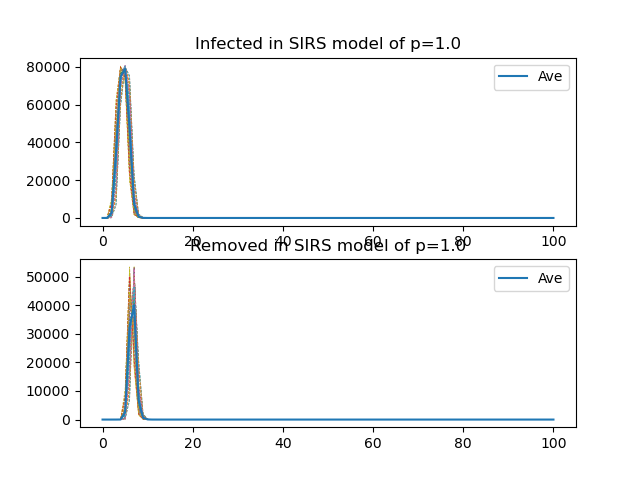
\includegraphics[scale=0.8]{sirsp10r1i3s3}
  \caption[SIRS p=1.0,r=1,i=3,init infected=3]{SIRS Model with p=1.0 r=1 i=3 initial infected=3 simulation using Snap.py}
  \end{figure}
  \begin{figure}
  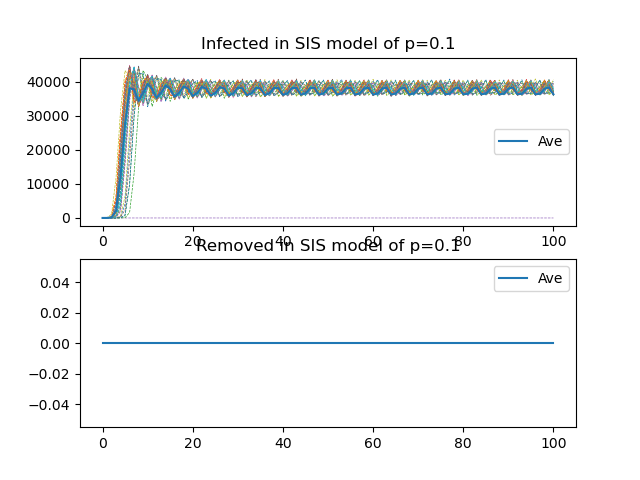
\includegraphics[scale=0.8]{sisp01r1i3s3}
  \caption[SIS p=0.1,r=1,i=3,init infected=3]{SIS Model with p=0.1 r=1 i=3 initial infected=3 simulation using Snap.py}
  \end{figure}
  \begin{figure}
  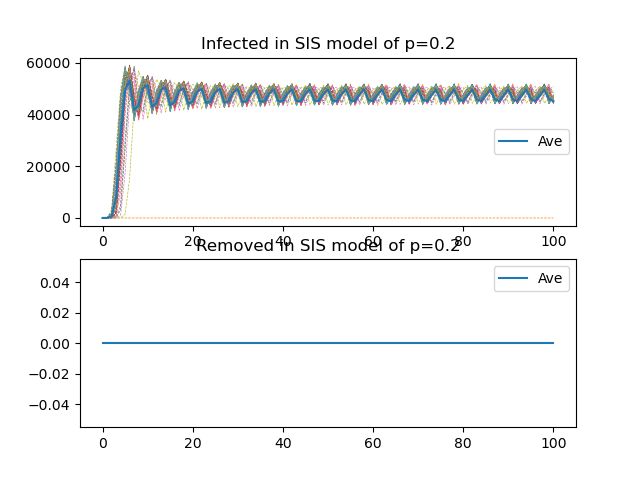
\includegraphics[scale=0.8]{sisp02r1i3s3}
  \caption[SIS p=0.2,r=1,i=3,init infected=3]{SIS Model with p=0.2 r=1 i=3 initial infected=3 simulation using Snap.py}
  \end{figure}
  \begin{figure}
  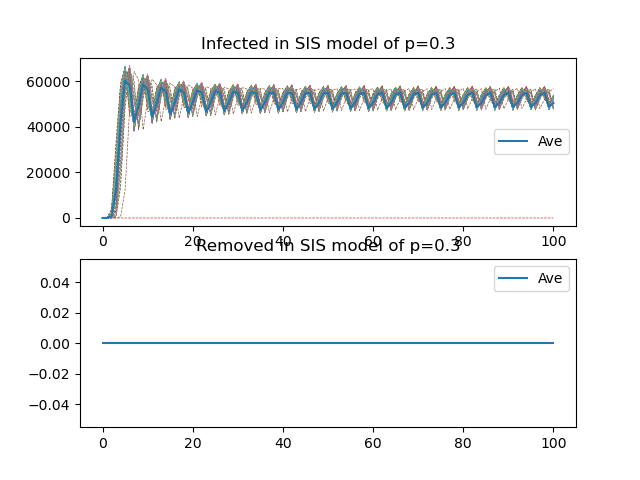
\includegraphics[scale=0.8]{sisp03r1i3s3}
  \caption[SIS p=0.3,r=1,i=3,init infected=3]{SIS Model with p=0.3 r=1 i=3 initial infected=3 simulation using Snap.py}
  \end{figure}
  \begin{figure}
  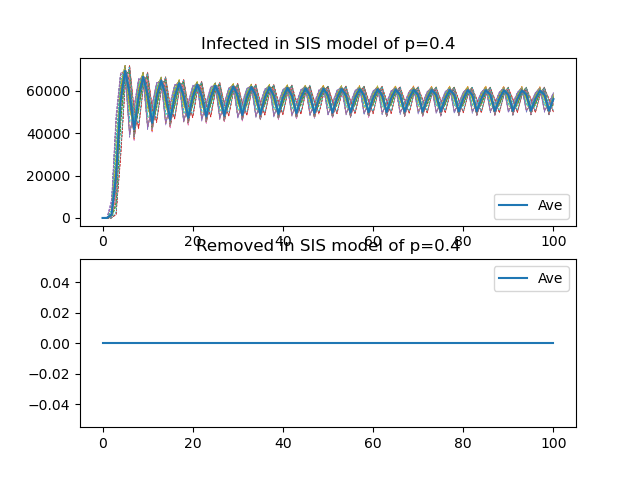
\includegraphics[scale=0.8]{sisp04r1i3s3}
  \caption[SIS p=0.4,r=1,i=3,init infected=3]{SIS Model with p=0.4 r=1 i=3 initial infected=3 simulation using Snap.py}
  \end{figure}
  \begin{figure}
  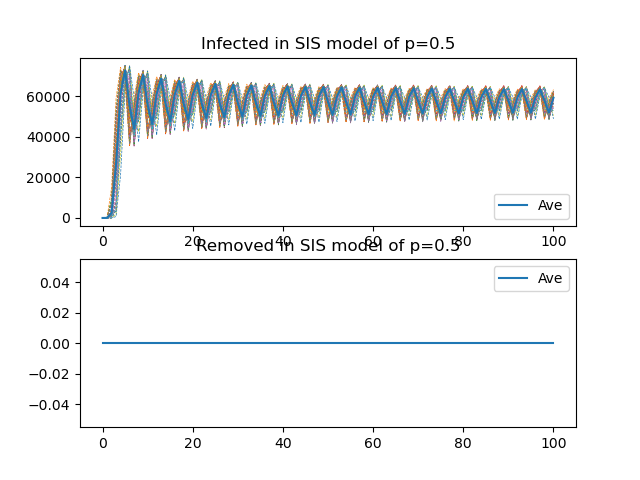
\includegraphics[scale=0.8]{sisp05r1i3s3}
  \caption[SIS p=0.5,r=1,i=3,init infected=3]{SIS Model with p=0.5 r=1 i=3 initial infected=3 simulation using Snap.py}
  \end{figure}
  \begin{figure}
  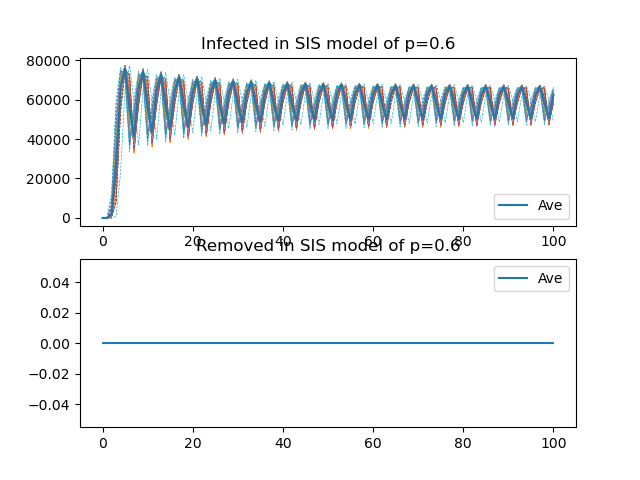
\includegraphics[scale=0.8]{sisp06r1i3s3}
  \caption[SIS p=0.6,r=1,i=3,init infected=3]{SIS Model with p=0.6 r=1 i=3 initial infected=3 simulation using Snap.py}
  \end{figure}
  \begin{figure}
  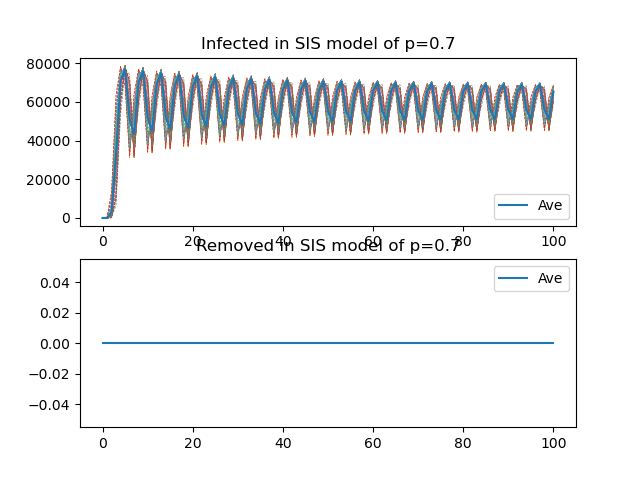
\includegraphics[scale=0.8]{sisp07r1i3s3}
  \caption[SIS p=0.7,r=1,i=3,init infected=3]{SIS Model with p=0.7 r=1 i=3 initial infected=3 simulation using Snap.py}
  \end{figure}
  \begin{figure}
  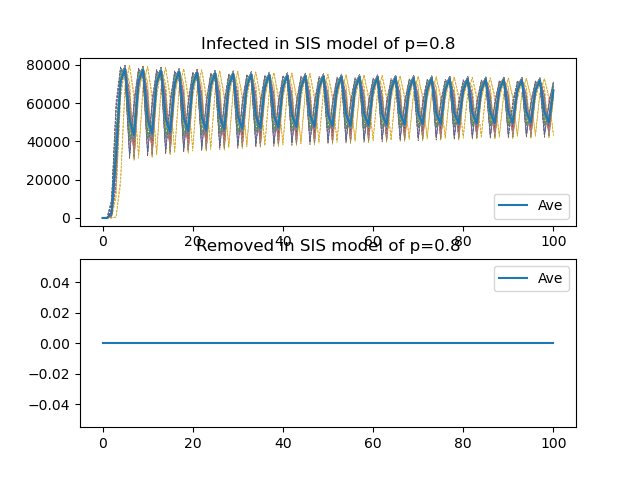
\includegraphics[scale=0.8]{sisp08r1i3s3}
  \caption[SIS p=0.8,r=1,i=3,init infected=3]{SIS Model with p=0.8 r=1 i=3 initial infected=3 simulation using Snap.py}
  \end{figure}
  \begin{figure}
  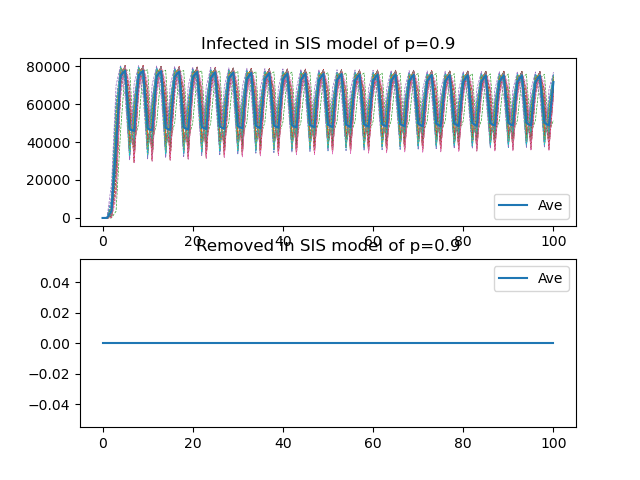
\includegraphics[scale=0.8]{sisp09r1i3s3}
  \caption[SIS p=0.9,r=1,i=3,init infected=3]{SIS Model with p=0.9 r=1 i=3 initial infected=3 simulation using Snap.py}
  \end{figure}
  \begin{figure}
  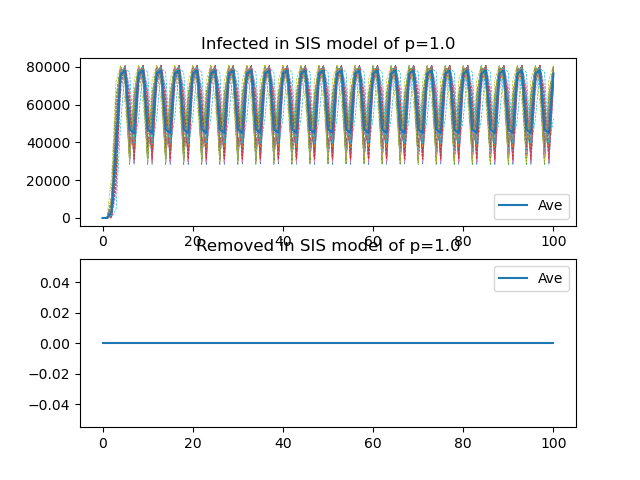
\includegraphics[scale=0.8]{sisp10r1i3s3}
  \caption[SIS p=1.0,r=1,i=3,init infected=3]{SIS Model with p=1.0 r=1 i=3 initial infected=3 simulation using Snap.py}
  \end{figure}

  \clearpage
\end{document}
